\subsection{Prediction of bug lifespan} % (fold)
\label{sub:Prediction of bug lifespan}

{\bf Task.} The lifespan of a bug is from the time it was reported until it was marked as closed. Essentially it means that is how much time it took to solve the bug. We wondered if it's at all possible to predict how long it will take to solve a bug by looking at its contents and metadata. The idea is that the longer and more complicated the description of the bug, the longer it would take to solve it.

{\bf Attributes used.} After inspecting the available data, we came to the conclusion that in addition to title and description other attributes such as priority, assigned developer, component, stars (indicates popularity) and type should be used. Status does not seem to make sense in this context since it is changed after a bug is closed.

{\bf Training data.} Training data consists of all those bugs that have been closed so that it's possible to calculate the lifespan by substracting the opened date from the closed date. The prediction outcome should be the lifespan as a timespan in milliseconds of a bug.

{\bf Text processing.} Text processing was done exactly like described in the previous section.

{\bf Performance.} Error rates are used to estimate accuracy of predictors. We are using a small sample size and only 3-fold stratified cross validation because the predictors take a long time to run. Error rates are given in milliseconds as the root of mean squared error.
\\
\\
\begin{tabular}{|c|c|p{8cm}|}
\hline
 Algorithm    & Sample Size &  Error Rate   \\
\hline
\hline
Linear Regression     &  50 & 15809561072.876 (183 days) +/- 1913382829.648 (22 days) \\
                      &  80 &  23016235402.190 (266 days) +/- 9169804778.729 (106 days) \\
Polynomial Regression &  50 &  12954847042.251 (150 days) +/- 5225235366.410 (60.5 days) \\
                      &  80 &  15726486894.414 (182 days) +/- 8349272014.051 (97 days) \\
\hline
\end{tabular}
\\
\\

{\bf Conclusion.} It took a lot of time for these data mining tasks to run so we were able to test them only on a small sample size. The obtained results were not very convincing nor useful.

\begin{figure}
\begin{center}
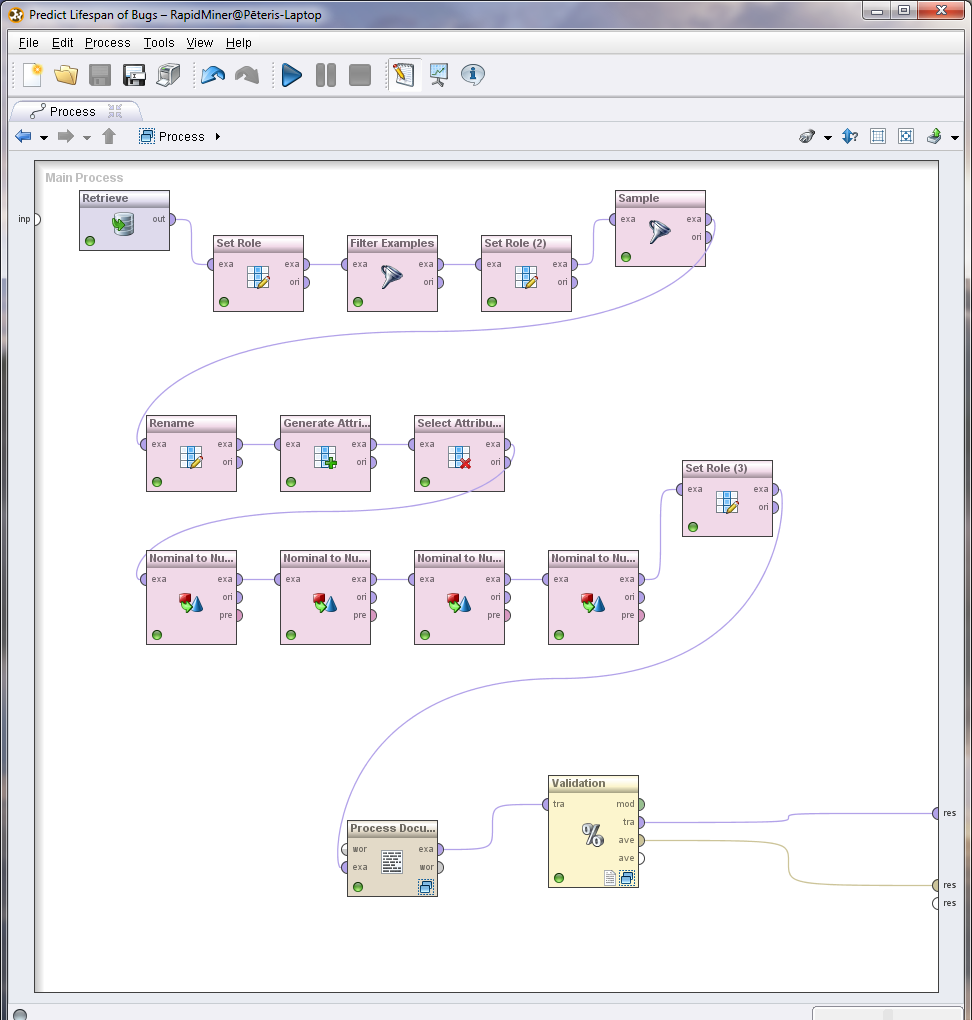
\includegraphics[scale=0.5]{ml3_prediction_workflow}
\caption{Workflow in Rapid Miner: 1. Load data 2-4. Filter non closed bugs 5. Use a sample 6-7. Calculate new Lifespan attribute 8. Select attributes 9-12. Convert polynominal to numeric attributes 13. Mark Lifespan attribute as label 14. Text processing 15. Cross validation }
\end{center}
\end{figure}
        
% subsection Prediction of bug lifespan (end)
